\chapter{Knot selection in spline models: cannabis dependence}
\label{applications-splines_knot_loc}

The meta-analysis of data from systematic review of the prevalence of cannabis dependence has a clear age-pattern, providing an example of the importance of knot selection in spline models.

Symptoms associated with cannabis dependence are compulsive use and difficulty with abstinence.  The American Psychiatric Association recognizes cannabis dependence as fulfilling three of the following seven criteria:
    \begin{itemize}
        \item tolerance
        \item withdrawal
        \item substance is taken in larger amounts or over longer period than intended
        \item persistent desire or unsuccessful efforts to control substance use
        \item great deal of time is spent to obtain use or recover from effects of substance
        \item important social, occupational or recreational activities are reduced because of substance use
        \item continued substance use despite knowledge of physiological or psychological problems induced by substance use \cite{american_diagnostic_2000, coffey_cannabis_2002}
    \end{itemize}

There is little data available on cannabis dependence.  Thirteen studies were identified for cannabis dependence prevalence, covering 6 countries (Figure \ref{fig:app-cannabis_data}).

    \begin{figure}[h]
        \begin{center}
            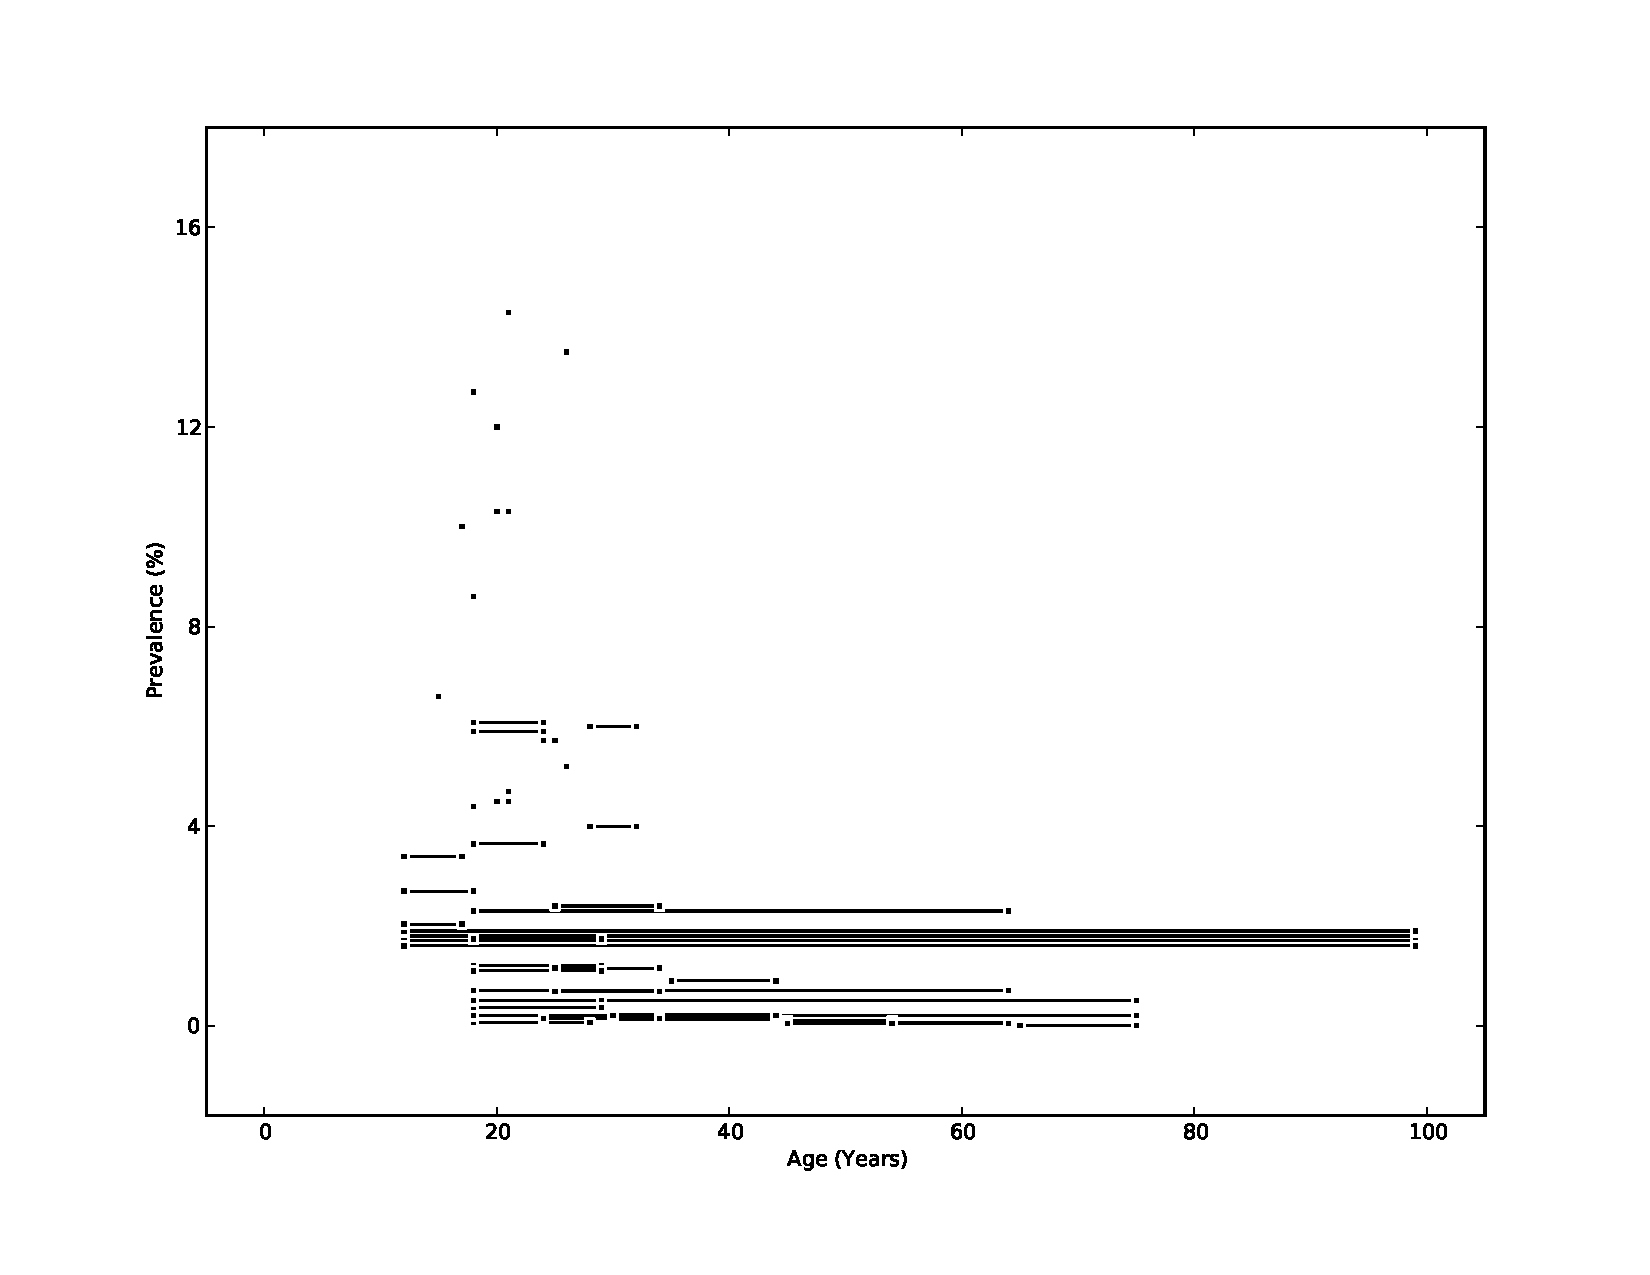
\includegraphics[width=\textwidth]{cannabis_dependence-data.pdf}
            \caption{Global data for cannabis dependence.}
            \label{fig:app-cannabis_data}
        \end{center}
    \end{figure}

As discussed in Chapter \ref{theory-age_pattern_model}, age-specific hazards are modeled with spline models.  A spline model is any piecewise polynomial function.  Knots partition the age range into intervals.  With ample data and clear age patterns, models will not be very sensitive to choice of knots.  However, when working with sparse and noisy data, the number and location of knots are important decisions as they can influence the model results substantially.  When this is the case, the number of knots and locations should be chosen a priori using expert knowledge concerning the disease being modeled.

The original model for cannabis dependence has knots at 0, 13, 17, 22, 30, 35, 40, 45, 50, 60, and 100.  The `less knot' model limits knots to ages 0, 13, 25, 65, and 100.   During the critical period of 13-50 years, the `more knot' model has knots every three years \{0, 13, 16, 19, \ldots, 43, 46, 49\} with additional knots at \{55, 60, 80, 100\}.  As seen in Figure \ref{fig:app-cannabis_knots}, choosing too few or too many knots can influence the model substantially.

    \begin{figure}[h]
        \begin{center}
            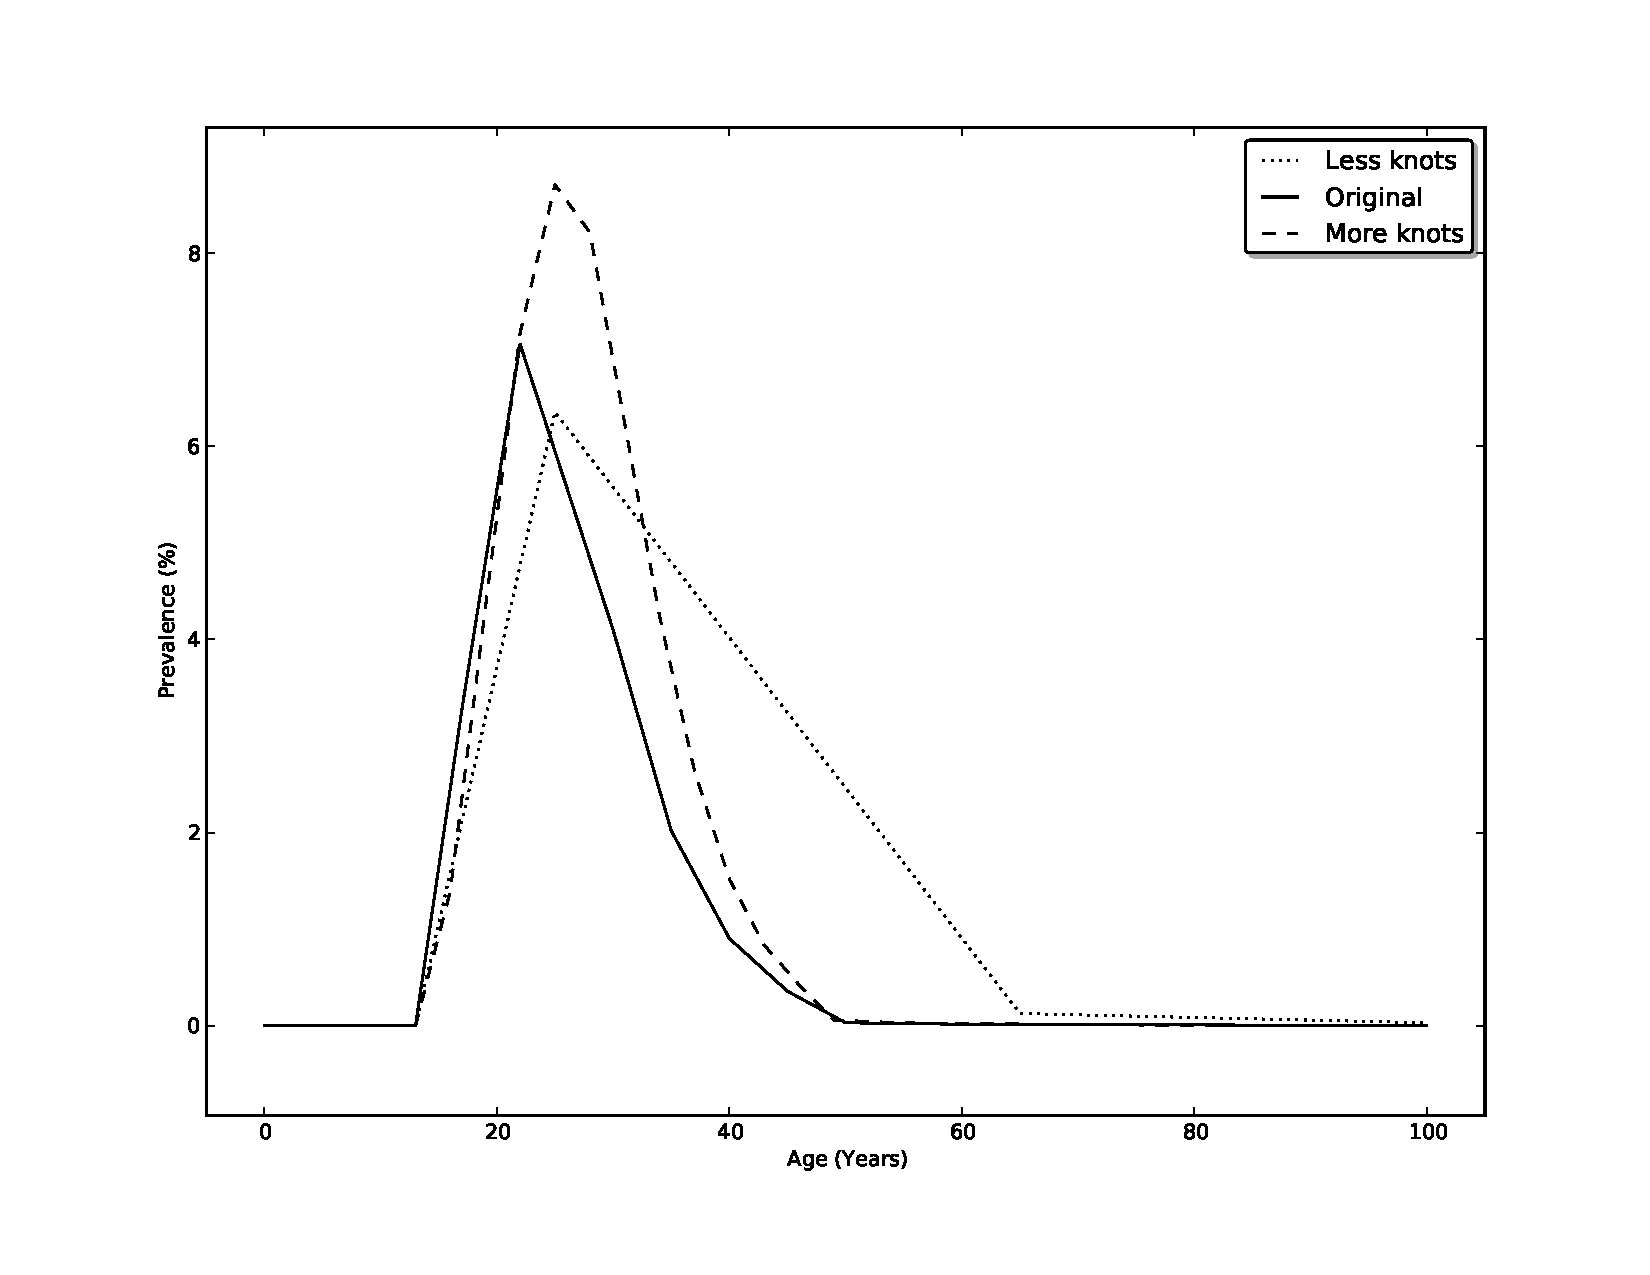
\includegraphics[width=\textwidth]{applications/cannabis_dependence-knots.pdf}
            \caption{Prevalence estimates of cannabis dependence in the original model and models with less and more knots.  All models use a single rate type model. }
        \label{fig:app-cannabis_knots}
        \end{center}
    \end{figure}

A penalized spline model with a smoothing parameter is another solution to knot selection.  The model includes more knots but adds a penalty to discourage the model from using more knots than necessary for the data.  The smoothing parameter controls the roughness of the estimating function and the fidelity of the data, making knot selection less influential as shown in Figure \ref{fig:app-cannabis_smoothing}.  However, too much smoothing and the overcompression of the prevalence estimates is not representative of the data.

    \begin{figure}[h]
        \begin{center}
            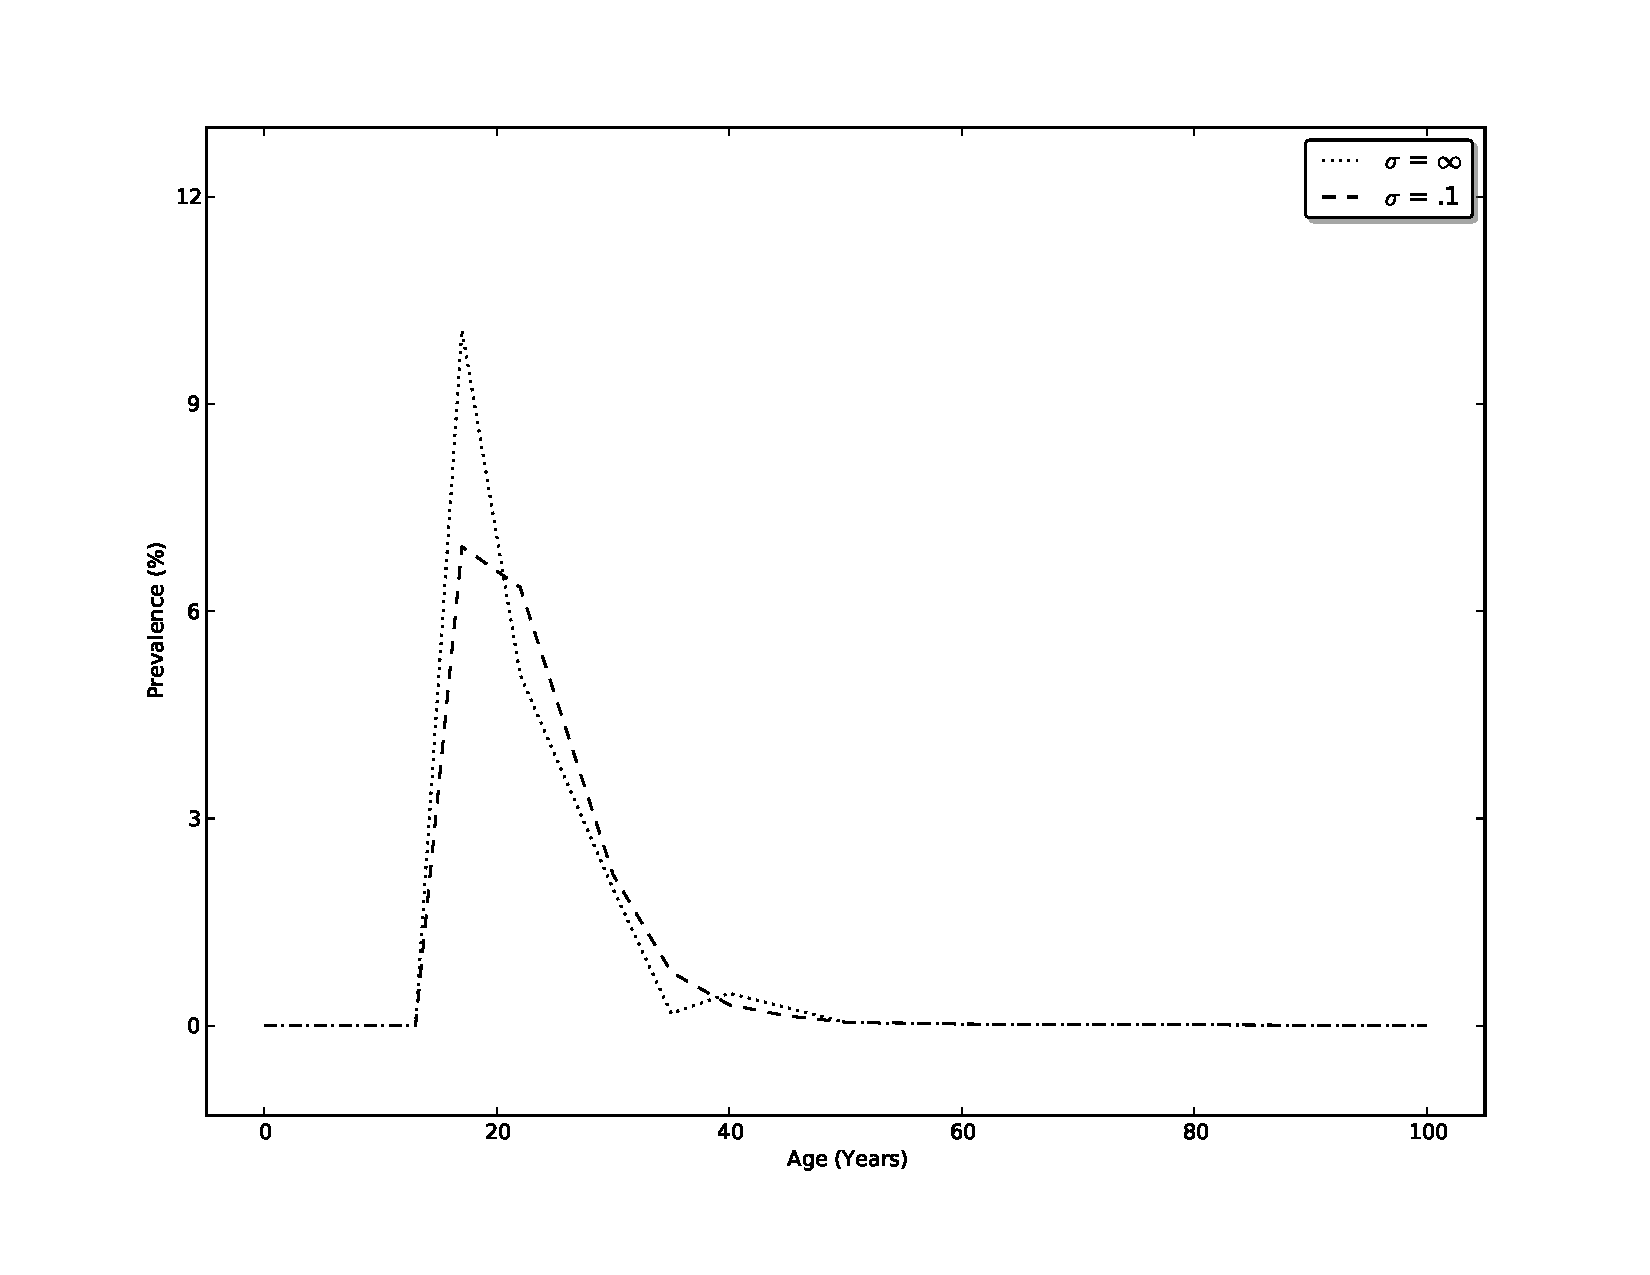
\includegraphics[width=\textwidth]{applications/cannabis_dependence-smoothing.pdf}
            \caption{Original model and a penalized spline model with a smoothing parameter $\sigma$. }
        \label{fig:app-cannabis_smoothing}
        \end{center}
    \end{figure}

